\chapter{Distributed Quantum Computing}
\label{chap:Distributed}

As we discussed in \S\ref{Hardware}, there are different approaches on how to build quantum computers. Now that many of these have been experimentally demonstrated, having built small quantum computers, the question of how to scale up is increasingly relevant. This has led to the proposal of distributed architectures~\citep{ArchitectureSurvey}.

In classical computing, an standard example of a distributed computer is the Non-Uniform Memory Access (NUMA) architecture: A system of independent computing nodes, each having its own local memory. In order to collaborate to perform an overall computation, the different nodes will need to communicate. In NUMA, they do so by accessing each other's memory. While nodes can manage their own local memory efficiently, accessing another node's memory is slow. Hence, we always attempt to minimise the amount of communication between nodes. A distributed quantum computer would follow the same principles, where each quantum processing unit (QPU) would own a collection of qubits (its local memory) and may access another QPU's qubits at the cost of some overhead, using entanglement.

\section{Communication through entanglement}
\label{Ebits}

For a QPU to be able to access another's qubit, we must provide them with some sort of communication channel. Simply using a classical channel (sending bits) is not helpful: the whole point of representing the state of the computation in qubits is that they may be in a superposition of classical states, which would take up to an exponential amount of space and processing on classical bits. We could consider physically transporting the system that encodes the qubit from one QPU to another, and while that is certainly possible with photons, in general it is not feasible to have a channel that is both fast and protects well against information loss due to decoherence.

In \S\ref{Principles}, we explained it was possible to affect a distant qubit by acting on another qubit with which it was entangled. We wish to exploit this property in order to allow a QPU to query another's QPU qubit. There are different levels of how strong a pair of qubits is entangled -- intuitively, how much they affect each other. This is often formalised as the correlation between the qubits possible measurement outcomes; for instance, the pair of qubits \(\frac{1}{\sqrt{2}}\ket{0,0} + \frac{1}{\sqrt{2}}\ket{1,1}\) is said to be \textit{maximally entangled}, as the possible measurement outcomes are exclusively either \(\ket{0,0}\) or \(\ket{1,1}\), always matching in both qubits\footnote{\, In total, there are four \textit{maximally entangled} states of a pair of qubits: \(\frac{1}{\sqrt{2}}\ket{0,0} + \frac{1}{\sqrt{2}}\ket{1,1}\) and \(\frac{1}{\sqrt{2}}\ket{0,0} - \frac{1}{\sqrt{2}}\ket{1,1}\) give perfect correlation, while \(\frac{1}{\sqrt{2}}\ket{0,1} + \frac{1}{\sqrt{2}}\ket{1,0}\) and \(\frac{1}{\sqrt{2}}\ket{0,1} - \frac{1}{\sqrt{2}}\ket{1,0}\) give perfect anti-correlation}. Naturally, the most efficient communication channel will take advantage of entanglement in its strongest form, and so we will make use pairs of qubits entangled in this particular maximally entangled state. This qubit pair configuration is generally known as a Bell state, and Figure~\ref{fig:bell} shows how to prepare it.

\begin{figure}
  \hspace*{20mm}
  \begin{tikzpicture}
    \node[inner sep=0pt] (circuit) at (0,0) {\includegraphics[scale=2]{Figures/circuits/Bell}};
    \node[right=8mm of circuit.north west, font=\itshape] (text) {a)};
  \end{tikzpicture} 
  \begin{tikzpicture}
    \node[inner sep=0pt] (circuit) at (0,0) {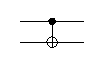
\includegraphics[scale=2, trim={5mm 0 0 0},clip]{Figures/circuits/CNOT}};
    \node[rectangle, fill=white, minimum size=5mm] (clear) at (-5mm,-5mm) {};
    \pic (e1) {ebit=e1/5.63mm/13mm};
    \node[right=2mm of circuit.north west, font=\itshape] (text) {b)};
  \end{tikzpicture}
\caption{Generation of the Bell state \(\ket{\Phi^+} = \frac{1}{\sqrt{2}}\ket{0,0} + \frac{1}{\sqrt{2}}\ket{1,1}\) shown in \textit{a)}. Its shorthand circuit notation is given in \textit{b)}.}
\label{fig:bell}
\end{figure}

An interesting property of the Bell state is shown in Figure~\ref{fig:sliding}: if a quantum gate, whose matrix representation is symmetric, is applied to one of the qubits, it is the same as if the gate was applied to the other qubit. In some sense, the gate can `slide' through the entanglement, like beads on a string; as if the entangled state were a curved wire, connecting the pair of qubits. Hopefully, this serves as a first intuition of how Bell states are a natural choice for implementing quantum comunication.

\begin{figure}
  \hspace*{30mm}
  \begin{tikzpicture}
    \node[inner sep=0pt] (circuit) at (0,0) {\includegraphics[scale=2, trim={0 0 5mm 0},clip]{Figures/circuits/H_I}};
    \pic (e1) {ebit=e1/5.63mm/13mm};
    \node[right=2mm of circuit.north west, font=\itshape] (text) {a)};
  \end{tikzpicture} 
  \hspace*{10mm}
  \begin{tikzpicture}
    \node[inner sep=0pt] (circuit) at (0,0) {\includegraphics[scale=2, trim={0 0 5mm 0},clip]{Figures/circuits/I_H}};
    \pic (e1) {ebit=e1/5.63mm/13mm};
    \node[right=2mm of circuit.north west, font=\itshape] (text) {b)};
  \end{tikzpicture}
\caption{Applying a gate on a Bell state. The circuits shown in \textit{a)} and \textit{b)} are equivalent.}
\label{fig:sliding}
\end{figure}

\subsection{Entanglement distillation}
\label{Distillation}

So far, we have explained how to generate a Bell state \(\ket{\Phi} = \frac{1}{\sqrt{2}}\ket{0,0} + \frac{1}{\sqrt{2}}\ket{1,1}\) inside a QPU (as in Figure~\ref{fig:bell}). However, what we aim for is that two different QPUs each own one of the qubits from \(\ket{\Phi}\). The challenge is then to send one of the qubits to another QPU, while preserving the state. The problem of sharing a Bell state between two parties is solved by the \textit{entanglement distillation} protocol~\citep{DistillationProtocol}, which ensures the shared pair of qubits are in the Bell state, up to some small error factor. In this section, we will give a brief explanation of how this protocol works.

In practice, there are no perfect communication channels. This means that it is impossible to send a quantum state without potentially altering it, introducing errors. And, as we mentioned earlier in \S\ref{Challenges}, detecting and correcting errors in quantum information is particularly challenging. Fortunately, in our case there is an easy way around it. We can create multiple \(\ket{\Phi}\) states in the first QPU, and send one of the qubits of each of these pairs to the second QPU, through a noisy channel. Then, we would have shared multiple imperfect \(\ket{\Phi}\) pairs, whose fidelity we can improve by making them interact with each other, destroying some of the pairs in the process. Before going into details on how we perform these interactions, we need some definitions:

\begin{itemize}
  \item \textit{Werner state}: It is the result of sending one of the qubits from \(\ket{\Phi}\) through a noisy channel characterised by a constant \(F \in [0,1]\). \(F\) determines the \textit{fidelity} of the channel, i.e.\ the probability that the qubit is sent without altering its state. Rather than an actual quantum state, the Werner state is a probability distribution of quantum states, known in the literature as a \textit{mixed state}. In particular, it is the probability distribution of actually having \(\ket{\Phi}\), with probability \(F\), having \(\ket{\Phi}\) with an \(X\) gate mistakenly applied to the sent qubit, or having \(\ket{\Phi}\) with a \(Z\) gate on it, or having \(\ket{\Phi}\) with both \(X\) and \(Z\) errors, each of these three cases\footnote{\, Although a channel will rarely introduce each of these errors with equal \(\frac{1-F}{3}\) probability, it is always possible to apply some local operations on each of the qubits so the probability distribution converges to that of the Werner state. Moreover, there may be channels that introduce errors other than \(X\) and \(Z\); however the resulting state after sharing \(\ket{\Phi}\) through any of these will always be some Werner state with some particular \(F\).} occurring with equal probability \(\frac{1-F}{3}\).

  \item \textit{Bilateral XOR (BXOR)}: Simply, two CNOT gates applied locally inside two different QPUs. Its intended use is to be applied to two Werner states; one QPU should have one of the qubits of each Werner state, and apply a CNOT on them, while the other should do the same on the other two qubits. Thus, one of the Werner states acts as control of the CNOTs, and the other as their target.
\end{itemize}

The entanglement distillation protocol takes a collection of Werner states and repeats the following three steps multiple times, until the fidelity of the Werner states is the one desired:

\begin{enumerate}
  \item Make pairs of two Werner states, and apply a BXOR to each pair. The new probability distribution (mixed state) on each of these four qubits is given in Table~\ref{tab:Werners}.

  \item For each pair of Werner states, measure the qubits corresponding to the Werner state that acted as the target of the BXOR -- this will require one measurement in each QPU. The outcome of the two measurements will match precisely in the cases where the fifth column of Table~\ref{tab:Werners} shows no \(X\) error. Examining the table, we can calculate the probability of that event to be: {\small \[T(F) = F^2 + \frac{2}{3} F(1-F) + \frac{5}{9} (1-F)^2\]}which, for \(F > \frac{1}{2}\), is always over a half.

  \item If the outcome of both measurements matched, keep the other two qubits (i.e.\ the control Werner state). Otherwise, discard them, not to be used again. Among the eight cases when we keep the Werner state, in two of them (grayed rows in Table~\ref{tab:Werners}) the state we keep has no errors, happening with probability: {\small \[P(F) = \frac{F^2 + 1/9(1-F)^2}{T(F)}\]}Thus, the kept qubit pairs are all Werner states with fidelity \(P(F)\) which, as shown in Figure~\ref{fig:fidelity}, is greater than \(F\) whenever \(F > \frac{1}{2}\).
\end{enumerate}

\begin{table}
\caption{Probability distribution defining a pair of Werner states, and the errors present in each case, before and after the BXOR is applied.}
\label{tab:Werners}
\scriptsize
\centering
\begin{tabular}{|c|cc|cc|c|}
\hline
\multicolumn{1}{|c|}{\multirow{2}{*}{Probability}} & \multicolumn{2}{c|}{Errors before} & \multicolumn{2}{c|}{Errors after} & \multicolumn{1}{c|}{\multirow{2}{*}{Kept?}} \\
\multicolumn{1}{|c|}{} & {\tiny Source} & {\tiny Target} & {\tiny Source} & {\tiny Target} & \multicolumn{1}{c|}{} \\
\hline
\rowcolor{gray!30}
\(F^2\) & -- & -- & -- & -- & \cmark \\ %THIS
\(\frac{1}{3}F(1-F)\) & -- & \(Z\) & \(Z\) & \(Z\) & \cmark \\
\(\frac{1}{3}F(1-F)\) & -- & \(X\) & -- & \(X\) & \\
\(\frac{1}{3}F(1-F)\) & -- & \(X,Z\) & \(Z\) & \(X,Z\) & \\
\(\frac{1}{3}F(1-F)\) & \(Z\) & -- & \(Z\) & -- & \cmark \\
\rowcolor{gray!30}
\(\frac{1}{9}(1-F)^2\) & \(Z\) & \(Z\) & -- & \(Z\) & \cmark \\ %THIS
\(\frac{1}{9}(1-F)^2\) & \(Z\) & \(X\) & \(Z\) & \(X\) & \\
\(\frac{1}{9}(1-F)^2\) & \(Z\) & \(X,Z\) & -- & \(X,Z\) & \\ 
\hline
\end{tabular}
\hspace{10pt}
\begin{tabular}{|c|cc|cc|c|}
\hline
\multicolumn{1}{|c|}{\multirow{2}{*}{Probability}} & \multicolumn{2}{c|}{Errors before} & \multicolumn{2}{c|}{Errors after} & \multicolumn{1}{c|}{\multirow{2}{*}{Kept?}} \\
\multicolumn{1}{|c|}{} & {\tiny Source} & {\tiny Target} & {\tiny Source} & {\tiny Target} & \multicolumn{1}{c|}{} \\
\hline
\(\frac{1}{3}F(1-F)\) & \(X\) & -- & \(X\) & \(X\) & \\
\(\frac{1}{9}(1-F)^2\) & \(X\) & \(Z\) & \(X,Z\) & \(X,Z\) & \\
\(\frac{1}{9}(1-F)^2\) & \(X\) & \(X\) & \(X\) & -- & \cmark \\
\(\frac{1}{9}(1-F)^2\) & \(X\) & \(X,Z\) & \(X,Z\) & \(Z\) & \cmark \\
\(\frac{1}{3}F(1-F)\) & \(X,Z\) & -- & \(X,Z\) & \(X\) & \\
\(\frac{1}{9}(1-F)^2\) & \(X,Z\) & \(Z\) & \(X\) & \(X,Z\) & \\
\(\frac{1}{9}(1-F)^2\) & \(X,Z\) & \(X\) & \(X,Z\) & -- & \cmark \\
\(\frac{1}{9}(1-F)^2\) & \(X,Z\) & \(X,Z\) & \(X\) & \(Z\) & \cmark \\
\hline
\end{tabular}
\end{table}

\begin{figure}
\centering
\begin{tikzpicture}
\begin{axis}[
    axis lines = left,
    xlabel = $F$,
    ylabel = {$P(F)$},     
    no markers,
    every axis plot/.append style={thick},
    every x tick label/.append style={font=\scriptsize},
    every y tick label/.append style={font=\scriptsize}]
\addplot[domain=0:1, samples=100, color=black!95]{(1 - x)^2/9 + x^2)/((5*(1 - x)^2)/9 + (2*(1 - x)*x)/3 + x^2};
\addplot[domain=0:1, samples=3, color=black!70, style=dashed]{x};
\end{axis}
\end{tikzpicture}
\caption{Fidelity after a single iteration of the distillation protocol, versus the original fidelity. The figure shows that \(F > \frac{1}{2} \, \Rightarrow \, P(F) > F\).}
\label{fig:fidelity}
\end{figure}

Figure~\ref{fig:fidelity} implies that we may use a communication channel as bad as to introduce errors slightly less than half of the times, and still generate a Werner state whose fidelity is arbitrarily close to one. Naturally, the more fidelity we wish to attain, and the worse the fidelity we start with is, more iterations of the protocol will be required. This increases the amount of time and resources -- number of initial Werner states -- we must pay in order to obtain a single entangled qubit pair.

Often in distributed quantum computing literature, a Bell state shared by two QPUs is known as an \textit{ebit} (entangled-bit) which, put another way, is just a Werner state with a fidelity close to one. Thus, this protocol produces ebits, which is the fundamental resource for quantum communication in distributed circuits. During the rest of this thesis, we use the term \textit{ebit half} to refer to any of the two qubits that comprise an ebit.

\section{Distributing circuits}
\label{IntroDistributing}

We now explain how ebits are used to allow a QPU to peek into another's qubits. Here, we will introduce the proposal of \citet{NonLocalCNOT}. Later on, in \S\ref{NonLocalGates}, we will extend this work with our own contributions. 

We aim to split a given circuit and distribute the fragments across multiple QPUs. The gates that should operate over qubits on different QPUs are known as \textit{non-local} gates. As we previously mentioned, any circuit can be converted to Clifford+T circuit (thanks to the Solovay-Kitaev theorem). In Clifford+T, the only gate that operates on more than one qubit is the CNOT. Hence, we only need to understand how CNOTs can be implemented non-locally.

The construction we will use is a slight variation of what was proposed by \citet{NonLocalCNOT}, and its scheme is shown in Figure~\ref{fig:nonlocalCNOT}. In principle, we will use an \textit{ebit} per non-local CNOT. We will call the QPU that holds the target qubit (the one with a \(\oplus\)) the `target QPU' and similarly for the control qubit. 

\begin{figure}
\begin{tikzpicture}
  \node[inner sep=0pt] (circuit) at (0,0) {\includegraphics[scale=2,trim={10mm 0 5mm 0},clip]{Figures/circuits/cnotToCut}};
  \coordinate[left=1mm of circuit.west] (leftPoint);
  \coordinate[right=1mm of circuit.east] (rightPoint);
  \pic (cut) {cut=leftPoint/rightPoint};
  \node[left=-2mm of circuit.north west, font=\itshape] (text) {a)};
  \node[font=\scriptsize\itshape, opacity=0.9, above right=3mm and -4mm of leftPoint] (QPUA) {QPU A};
  \node[font=\scriptsize\itshape, opacity=0.9, below right=3mm and -4mm of leftPoint] (QPUB) {QPU B};
\end{tikzpicture}
\hspace{3mm}
\begin{tikzpicture}
  \node[inner sep=0pt] (circuit) at (0,0) {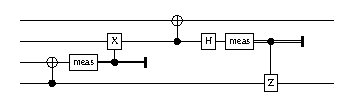
\includegraphics[scale=2]{Figures/circuits/nonlocalCNOT}};
  \pic (e1) {ebit=e1/12.7mm/13mm};
  \coordinate[left=-5.5mm of circuit.west] (leftPoint);
  \coordinate[right=-5.5mm of circuit.east] (rightPoint);
  \pic (cut) {cut=leftPoint/rightPoint};
  \pic [below left=27mm and -13mm of circuit.north west] (entangler) {opaquebox=entangler/9mm/55mm/23mm/41mm/cat-entangler};
  \pic [below left=27mm and -13mm of circuit.north west] (disentangler) {opaquebox=disentangler/9mm/105mm/23mm/39.5mm/cat-disentangler};
  \node[right=2mm of circuit.north west, font=\itshape] (text) {b)};
\end{tikzpicture}
\caption
{A non-local CNOT, shown in \textit{a)}. The dashed line indicates how the circuit is separated into two QPUs. The implementation scheme is given in \textit{b)}.}
\label{fig:nonlocalCNOT}
\end{figure}

The implementation of a local CNOT gate has three steps. First, we must apply what the authors refer to as the \textit{cat-entangler} (Figure~\ref{fig:cat-entangler}), which creates a local `copy'\footnote{\, Note that there is no such thing as `copying' a quantum state (due to the non-cloning theorem). What we mean here by `copying' is generating, from \(\ket{\psi} = \alpha\ket{0} + \beta\ket{1}\), the state \(\ket{\psi'} = \alpha\ket{0,0} + \beta\ket{1,1}\) which is fundamentally different from an actual copy: \(\ket{\psi}\otimes\ket{\psi} = \alpha^2\ket{0,0} + \alpha\beta\ket{0,1} + \alpha\beta\ket{1,0} + \beta^2\ket{1,1}\).} of the control qubit inside the target QPU. In the process, the ebit half in the control QPU is measured (and thus destroyed), and the outcome is used to correct the other half, in the same spirit as in the MBQC model. These corrections are done via \textit{classically controlled gates}; devices that either apply a transformation to the qubit or none, depending on the value of a classical bit. Notice that the only information physically crossing the boundary between blocks is the \textit{classical} outcome of the measurement (a bit, either \(0\) or \(1\)).

\begin{figure}
\centering
\begin{tikzpicture}
  \node[inner sep=0pt] (circuit) at (0,0) {\includegraphics[scale=2]{Figures/circuits/entangler}};
  \pic (e1) {ebit=e1/5.63mm/13mm};
  \coordinate[below left=10.7mm and 0mm of circuit.north west] (leftPoint);
  \coordinate[right=61mm of leftPoint] (rightPoint);
  \pic (cut) {cut=leftPoint/rightPoint};
  \node[font=\scriptsize\itshape, opacity=0.9, above right=3mm and -3mm of leftPoint] (QPUA) {QPU A};
  \node[font=\scriptsize\itshape, opacity=0.9, below right=3mm and -3mm of leftPoint] (QPUB) {QPU B};
\end{tikzpicture}
\caption{Implementation of the cat-entangler. An ebit is used to make the information in QPU \(B\)'s wire available to QPU \(A\). A doubled line indicates the wire holds classical information. Hence, the \(X\) gate is classically controlled, and the line that crosses the boundary represents classical communication. For any input state \(\alpha\ket{0} + \beta\ket{1}\), the output is \(\alpha\ket{0,0} + \beta\ket{1,1}\).}
\label{fig:cat-entangler}
\end{figure}

Then, the CNOT gate is \textit{applied locally} inside the target QPU, between its ebit half and the target qubit. At the end, the \textit{cat-disentangler} must be applied (Figure~\ref{fig:cat-disentangler}), which simply destroys -- with a measurement -- the remaining ebit half and then corrects the control qubit, so the randomness of the measurement is counteracted. Once again, only classical information crosses the boundary.

\begin{figure}
\centering
\begin{tikzpicture}
  \node[inner sep=0pt] (circuit) at (0,0) {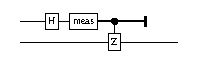
\includegraphics[scale=2]{Figures/circuits/disentangler}};
  \coordinate[below left=10.7mm and 0mm of circuit.north west] (leftPoint);
  \coordinate[right=61mm of leftPoint] (rightPoint);
  \pic (cut) {cut=leftPoint/rightPoint};
  \node[font=\scriptsize\itshape, opacity=0.9, above right=3mm and -3mm of leftPoint] (QPUA) {QPU A};
  \node[font=\scriptsize\itshape, opacity=0.9, below right=3mm and -3mm of leftPoint] (QPUB) {QPU B};
\end{tikzpicture}
\caption{Implementation of the cat-disentangler. Essentially, it destroys the ebit half (top wire) that the cat-entangler coupled with QPU B's wire. A doubled line indicates the wire holds classical information (a bit). For any input state \(\alpha\ket{0,0} + \beta\ket{1,1}\), the output is \(\alpha\ket{0} + \beta\ket{1}\).}
\label{fig:cat-disentangler}
\end{figure}

In this way, we have implemented a non-local CNOT gate using one ebit and two classical bit messages between QPUs. However, the true advantage of this approach is attained when multiple non-local CNOTs are implementing using a single ebit: Once the cat-entangler is applied, any number of CNOTs whose target is in the same QPU, and that are controlled by the same qubit, may all be implemented by using the same ebit half as control, as shown in Figure~\ref{fig:nonlocalCNOTs}.

\begin{figure}
\centering
\begin{tikzpicture}
  \node[inner sep=0pt] (circuit) at (0,0) {\includegraphics[scale=2]{Figures/circuits/nonlocalCNOTs}};
  \pic (e1) {ebit=e1/26.79mm/13mm};
  \pic [below left=27mm and -13mm of circuit.north west] (entangler) {box=entangler/23.5mm/52mm/23mm/38mm/Entangler/0mm/1mm};
  \pic [below left=27mm and -13mm of circuit.north west] (disentangler) {box=disentangler/23.5mm/126mm/23mm/38.5mm/Disentangler/10.5mm/1mm};
  \coordinate[below left=7mm and -6mm of circuit.west] (leftPoint);
  \coordinate[right=130.5mm of leftPoint] (rightPoint);
  \pic (cut) {cut=leftPoint/rightPoint};
  \node[font=\small\itshape, opacity=0.9, below right=7.7mm and -4.5mm of leftPoint] (W) {W};
\end{tikzpicture}
\caption{Implementing three non-local CNOTs using a single ebit. Wire \(W\) acts as control for the three of them. Only classical information crosses the boundary between QPUs, apart from the previously shared ebit.}
\label{fig:nonlocalCNOTs}
\end{figure}

Now, depending of how we choose to partition the circuit, there will be different groups of CNOTs that we may be able to implement using a single ebit. We will then wish to find the partition that requires the fewest ebits to implement all of its CNOT gates. This optimization problem is not discussed in the original paper, nor in any other work, as far as we know. It will be our main contribution in this thesis, along with an extension of the results just explained, both found in Chapter~\ref{chap:Project}.


\section{Distributed quantum architectures}
\label{DQC_Architecture} 

In this section we propose an abstract distributed quantum architecture. We claim that any distributed quantum computing technology will be characterised by the following features:

\begin{itemize}
  \item \textit{Multiple quantum processing units (QPUs)}: Each of the QPUs should be able to perform universal quantum computations on its collection of `workspace' qubits. It should be possible to prepare these qubits to hold the input data of a program, and read output from (measure) them. It should also be possible to apply classically controlled gates on qubits.

  \item \textit{Specialised space for ebits}: Each QPU should have some extra qubits meant to be used as ebit halves. These should be specialised so the operations necessary for ebit generation can be applied on them fast and reliably. The QPU should support the application of CNOTs (or some other suitable 2-qubit gate) between these specialised qubits and the ones in its workspace.
  
  \item \textit{Ebit generation hardware}: This includes the (noisy) quantum communication channel itself and the ability to perform the distilling process. The generation of ebits may be done either in a centralised manner, with an specialised device that creates Bell states and sends them to the different QPUs, or decentralised, each QPU having their own hardware for creating and sharing the ebits. Depending on the technology used, entanglement distillation may be more or less essential; for instance, if the step of sharing Bell states is done using quantum optics (photons), the quantum channel is likely to be fairly reliably, so it will only require a few iterations of the distilling process.
  
  \item \textit{Classical communication network}: Which will be required in the process of entanglement distillation, as well as to perform cat-entanglers and cat-disentanglers. The QPUs will send signals through the network when they measure their qubits, and read from it to apply corrections. 
\end{itemize}

As we discussed in \S\ref{Distillation}, there is a compromise between the quality of the ebits and the effort put into preparing them. Fortunately, \citet{NoisyChannels} showed that efficient distributed quantum computation using noisy ebits is feasible. Nevertheless, ebit generation will always be the main bottleneck of any distributed quantum architecture, as it is by far more expensive than classical communication and any local operation (in fact, multiple local operations are required in order to generate and use an ebit). Therefore, we will want to minimise the number of ebits required to implement any given algorithm.

\citet{DistributedQCHW} have proposed an experimental distributed quantum architecture. They explain how each of the features listed above may be implemented, particularly focusing on how entanglement across QPUs is achieved (ebit generation). Their proposal is to use cavities (traps) where the particles encoding the qubits are kept, and use laser pulses (photons) to entangle cavities of different QPUs together.